\section{Instruction templates}
\label{app:prompts}

\Tabref{tab:prompts} lists the four original instructions. Each prompt is the instruction, a blank line and the task input, prefixed with \texttt{Review:}, \texttt{Article:}, \texttt{Question:} (followed by lettered options) or \texttt{Passage:} \dots\ \texttt{Question:}. Words in the protected column are never changed by \syn or \typo edits.

\begin{table}[h]
\centering
\small
\renewcommand{\arraystretch}{1.2}
\begin{tabular}{@{}p{0.11\linewidth}p{0.63\linewidth}p{0.2\linewidth}@{}}
\toprule
\textbf{Task} & \textbf{Instruction (four sentences)} & \textbf{Protected words} \\
\midrule
\sst & You are an expert sentiment analysis assistant. Read the movie review provided below carefully. Determine whether the overall sentiment expressed in the review is positive or negative. Answer with exactly one word: positive or negative. & positive, negative \\
\agnews & You are an expert news topic classifier. Read the news article provided below carefully. Decide which topic the article belongs to; the possible topics are World, Sports, Business, and Sci/Tech. Respond with only the topic name and nothing else. & World, Sports, Business, Sci/Tech \\
\arc & You are a knowledgeable science tutor. Read the multiple-choice question provided below carefully. Choose the single best answer from the options. Respond with only the letter of the correct option (A, B, C, or D). & A, B, C, D \\
\squad & You are a precise reading comprehension assistant. Read the passage provided below carefully and then answer the question about it. The answer is a short span copied directly from the passage. Respond with only the answer span, without any explanation. & (none) \\
\bottomrule
\end{tabular}
\caption{Original instructions. Each has a persona sentence, a reading directive, a task definition and an output-format constraint.}
\label{tab:prompts}
\end{table}

\section{Implementation and reproducibility}
\label{app:impl}

We used llama.cpp \texttt{llama-server} (build b11624) on CPU with the Q8\_0 GGUF files \texttt{bartowski/Qwen2.5-1.5B-Instruct-GGUF} and \texttt{bartowski/Llama-3.2-1B-Instruct-GGUF}. Items were sampled with a fixed seed (42). The full run took about 2.3 hours of wall-clock time on up to four concurrent servers (6--8 threads each) on a shared 32-core host, with no API cost. In total we scored 2 models $\times$ 4 tasks $\times$ 26 conditions $\times$ 100 items $=$ 20,800 generations. We logged every prompt and response. Among 212 accidentally duplicated \squad requests for \llama, 95\% produced byte-identical outputs, which matches the noise floor in \tabref{tab:baselines}.

\section{Additional figures}
\label{app:figures}

\begin{figure}[h]
\centering
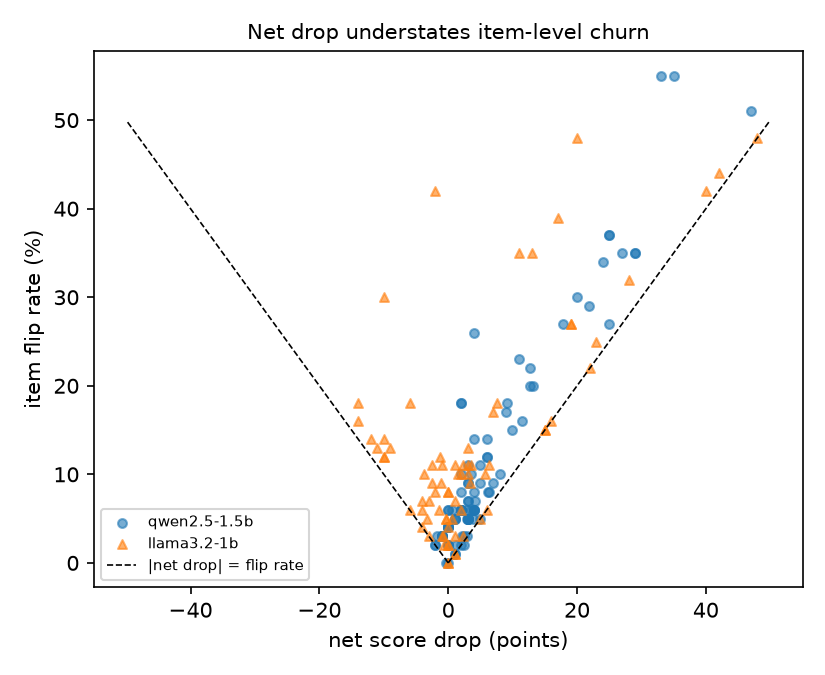
\includegraphics[width=0.55\linewidth]{figures/flip_vs_delta.png}
\caption{Item flip rate against net score drop for all 96 perturbed condition--task pairs of each model. Points on the dashed V have no churn beyond the net change. Most points lie well above it: edits fix some items while breaking others, so a small net change can hide a flip rate above 40\%.}
\label{fig:flip}
\end{figure}


\begin{figure}[h]
\centering
\begin{subfigure}[b]{0.49\textwidth}
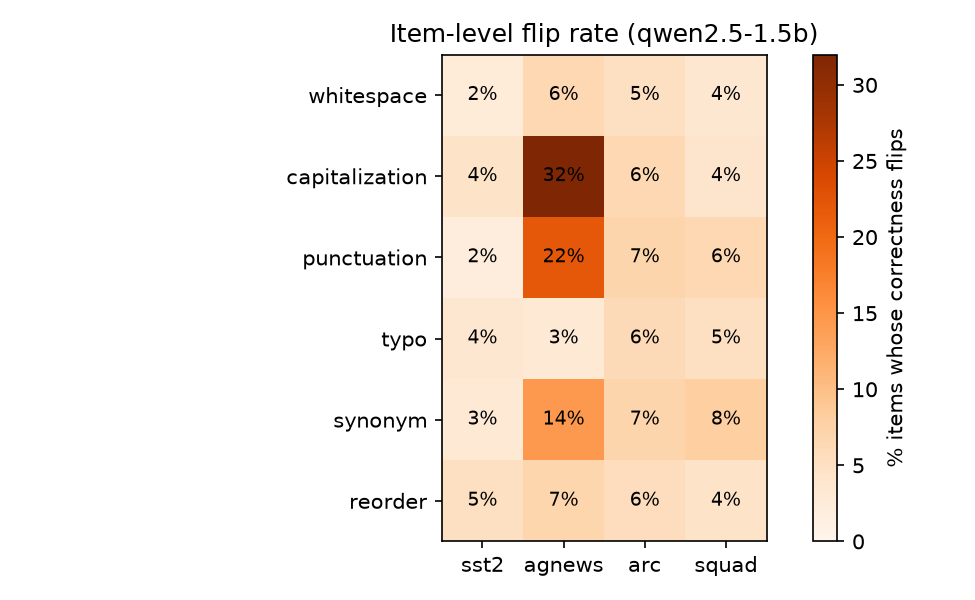
\includegraphics[width=\textwidth]{figures/heatmap_flip_qwen2_5-1_5b.png}
\caption{\qwen}
\end{subfigure}
\hfill
\begin{subfigure}[b]{0.49\textwidth}
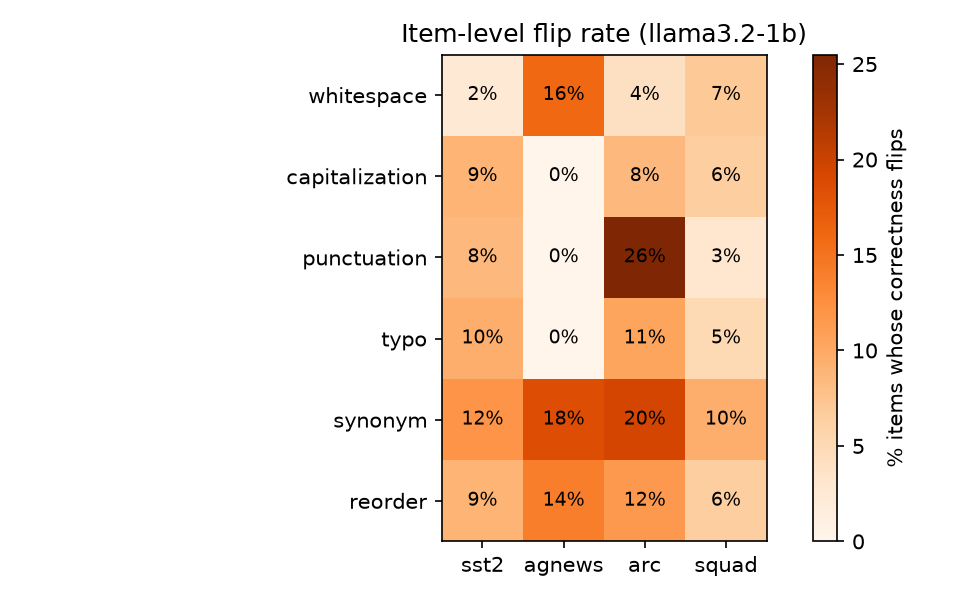
\includegraphics[width=\textwidth]{figures/heatmap_flip_llama3_2-1b.png}
\caption{\llama}
\end{subfigure}
\caption{Item flip rate for every condition and task. Flip rates are often several times larger than the net score change in \tabref{tab:h1}.}
\label{fig:heat_flip}
\end{figure}

\begin{figure}[h]
\centering
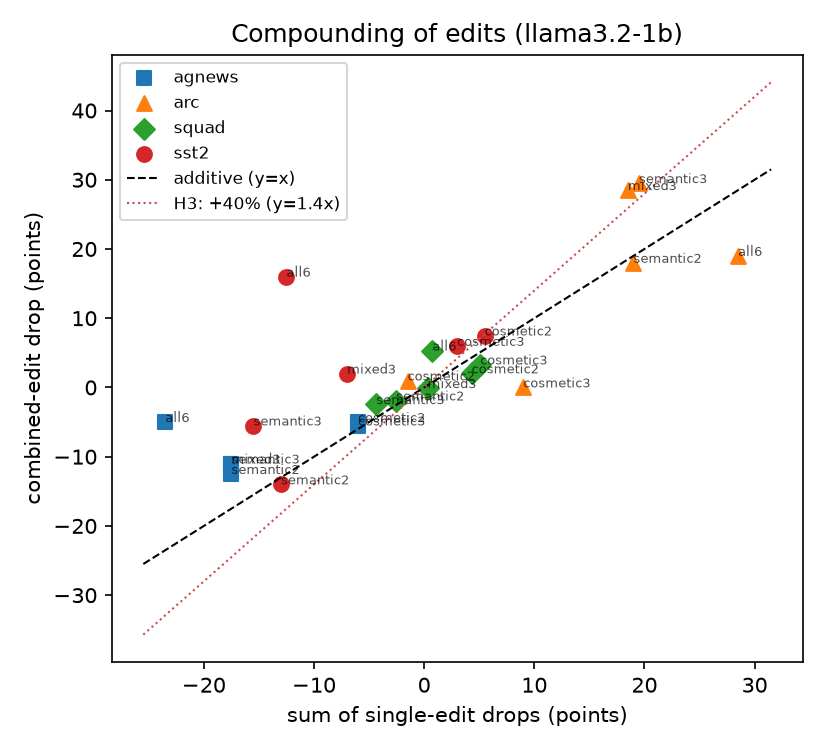
\includegraphics[width=0.6\linewidth]{figures/compounding_llama3_2-1b.png}
\caption{Drop of each combined edit against the sum of its parts for \llama. Because single-edit drops have mixed signs, the additive ratio is unstable for this model; \secref{sec:h3} reports the union-baseline analysis.}
\label{fig:h3_llama}
\end{figure}
